\section{Cấu hình Jenkins}
\label{sec:cau-hinh-jenkins}

\subsection{Cài đặt Jenkins trên AWS EC2}
Jenkins được cài đặt trên AWS EC2 instance và truy cập qua \texttt{http://3.27.92.213:8080}.

Các plugin cần thiết đã cài đặt:
\begin{itemize}[noitemsep]
    \item \textbf{GitHub Branch Source Plugin}: Hỗ trợ Multibranch Pipeline với GitHub
    \item \textbf{Pipeline Plugin}: Hỗ trợ Jenkinsfile declarative pipeline
    \item \textbf{JUnit Plugin}: Hiển thị kết quả test
    \item \textbf{Credentials Binding Plugin}: Quản lý secrets (SonarQube token, Snyk token)
    \item \textbf{Timestamps Plugin}: Hiển thị thời gian trong console output
\end{itemize}

\begin{figure}[H]
    \centering
    % CHỈ DẪN ẢNH: Thả ảnh 01-jenkins-dashboard.png vào thư mục img/
    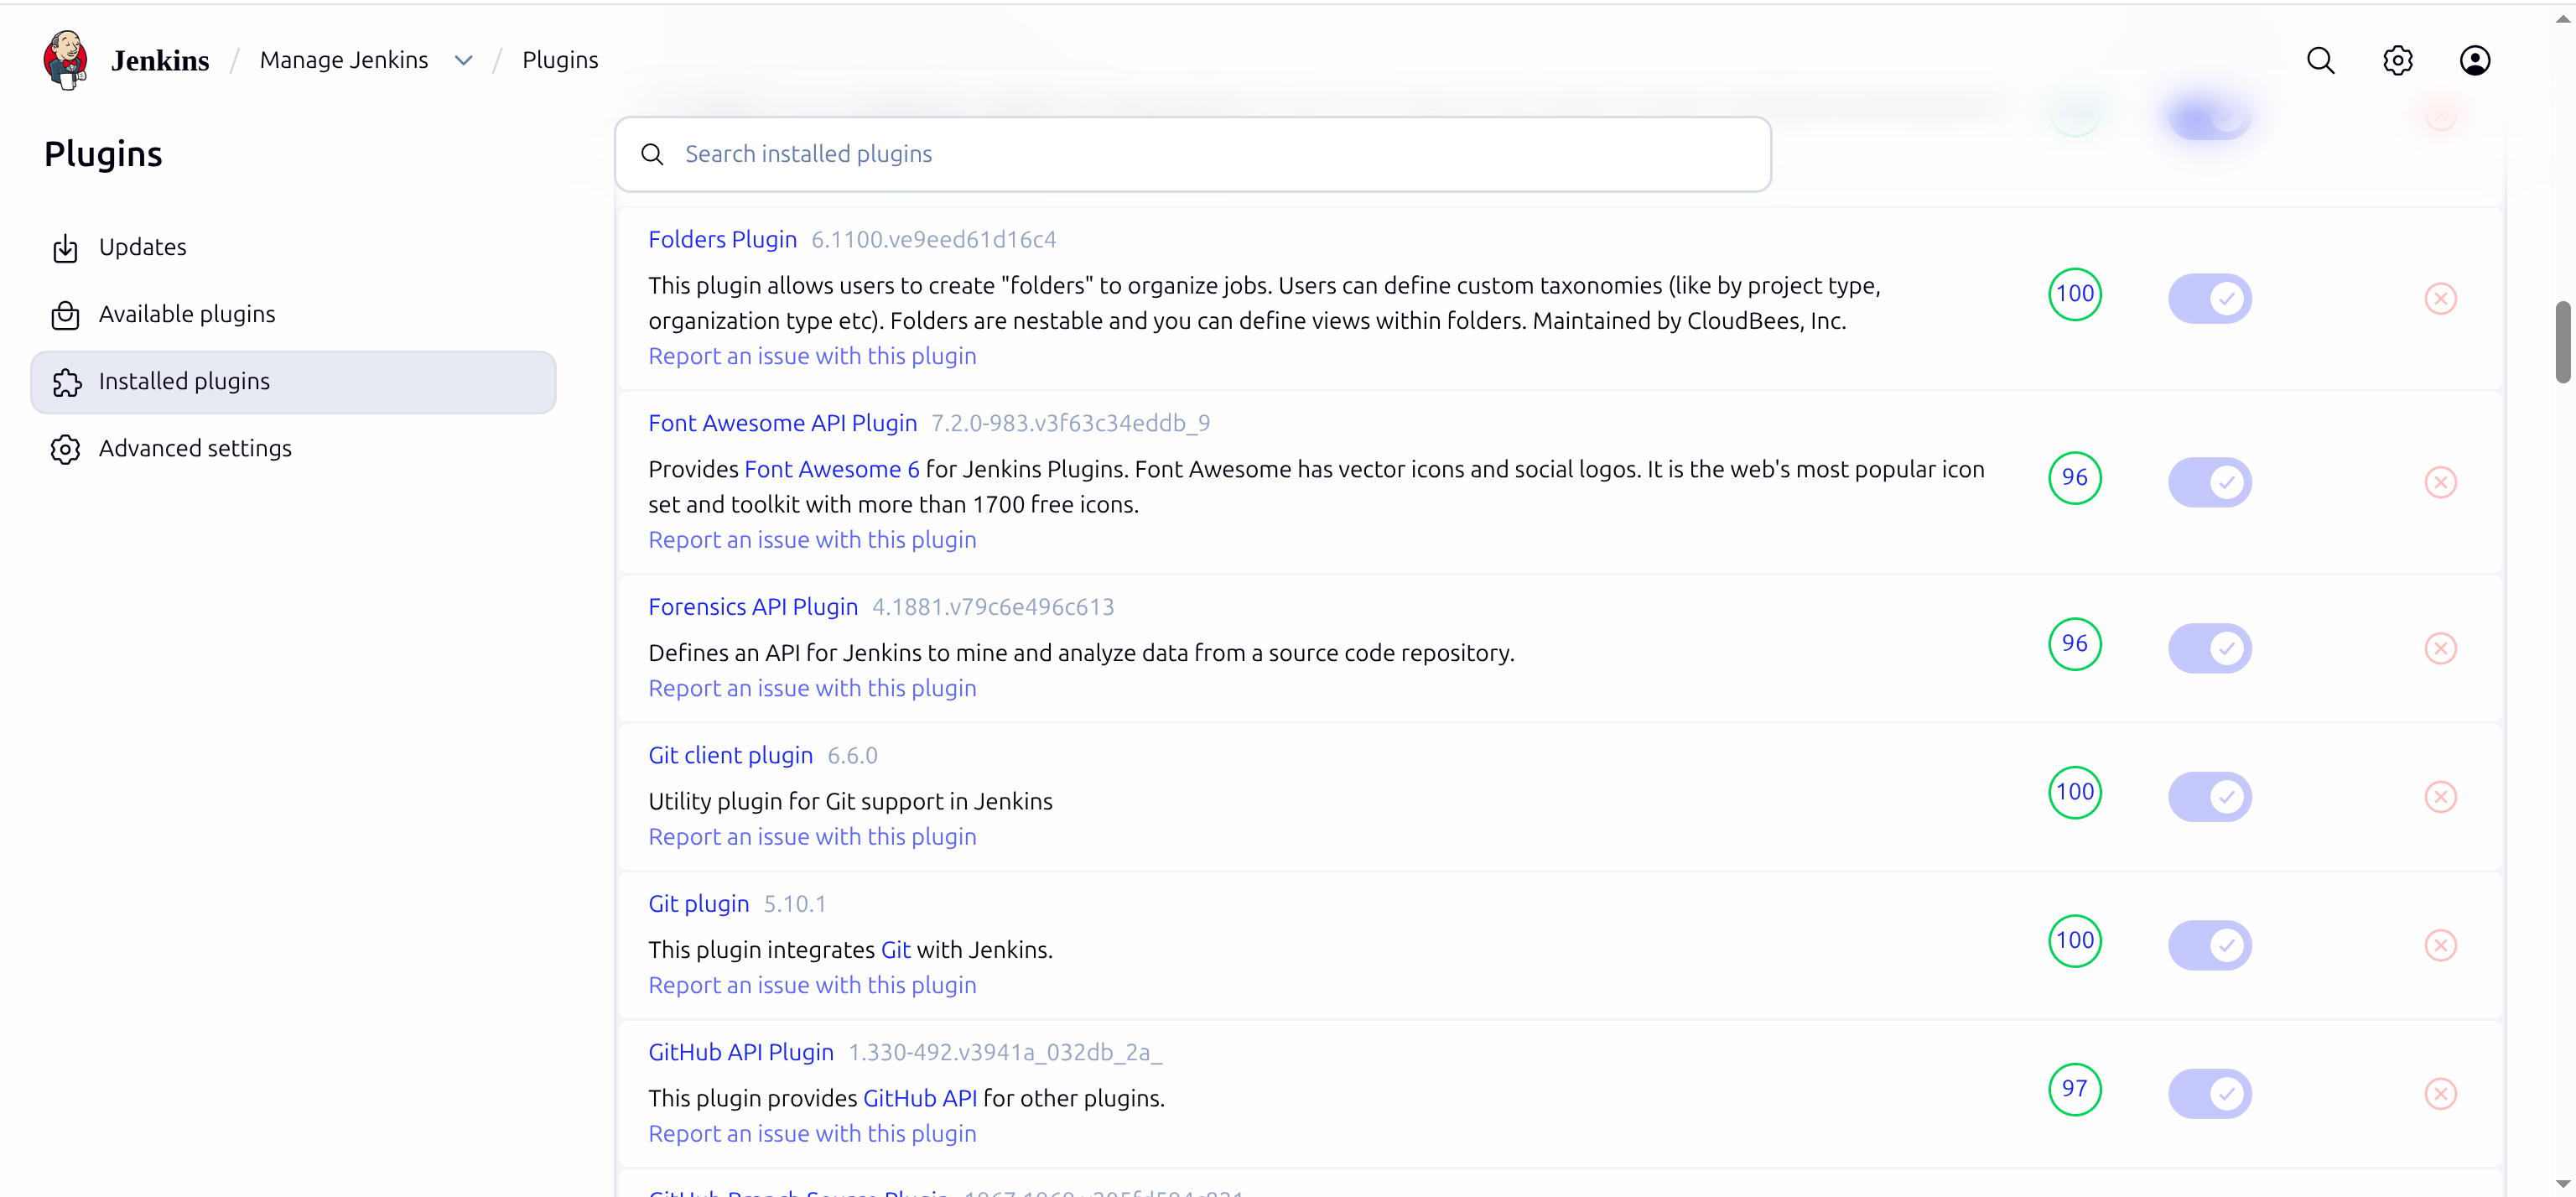
\includegraphics[width=0.9\textwidth]{img/01-jenkins-dashboard.png}
    \caption{Giao diện Dashboard quản lý Jenkins trên AWS EC2}
\end{figure}

\subsection{Cấu hình Tools}
Trong Jenkins Global Tool Configuration:
\begin{itemize}[noitemsep]
    \item \textbf{JDK}: Cấu hình JDK-25 (OpenJDK 25)
    \item \textbf{Maven}: Cấu hình Maven (Latest LTS)
\end{itemize}

\begin{figure}[H]
    \centering
    % CHỈ DẪN ẢNH: Thả ảnh 06-jenkins-tools-jdk.png vào thư mục img/
    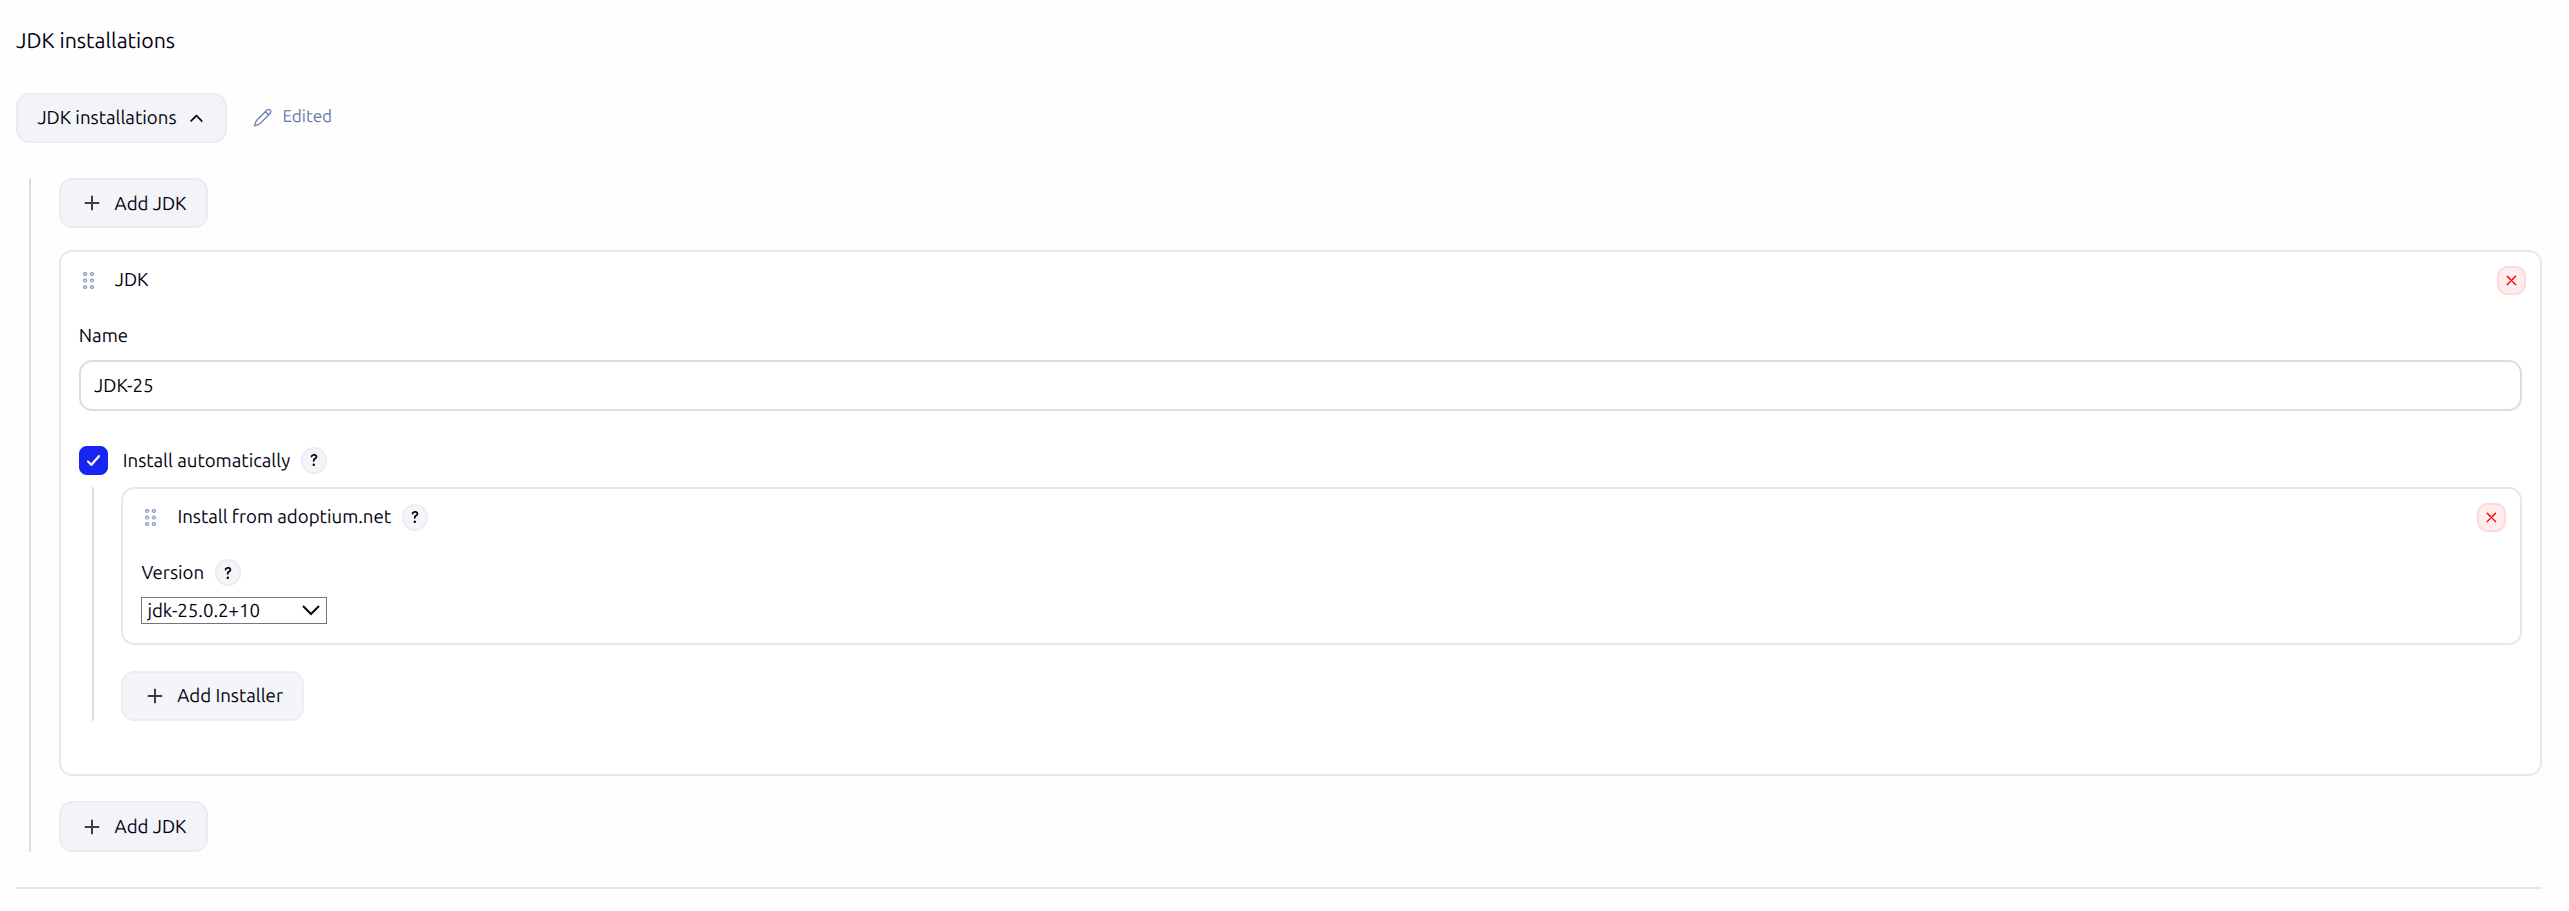
\includegraphics[width=0.9\textwidth]{img/06-jenkins-tools-jdk.png}
    \caption{Cấu hình JDK-25 trong Jenkins Global Tool Configuration}
\end{figure}

\begin{figure}[H]
    \centering
    % CHỈ DẪN ẢNH: Thả ảnh 07-jenkins-tools-maven.png vào thư mục img/
    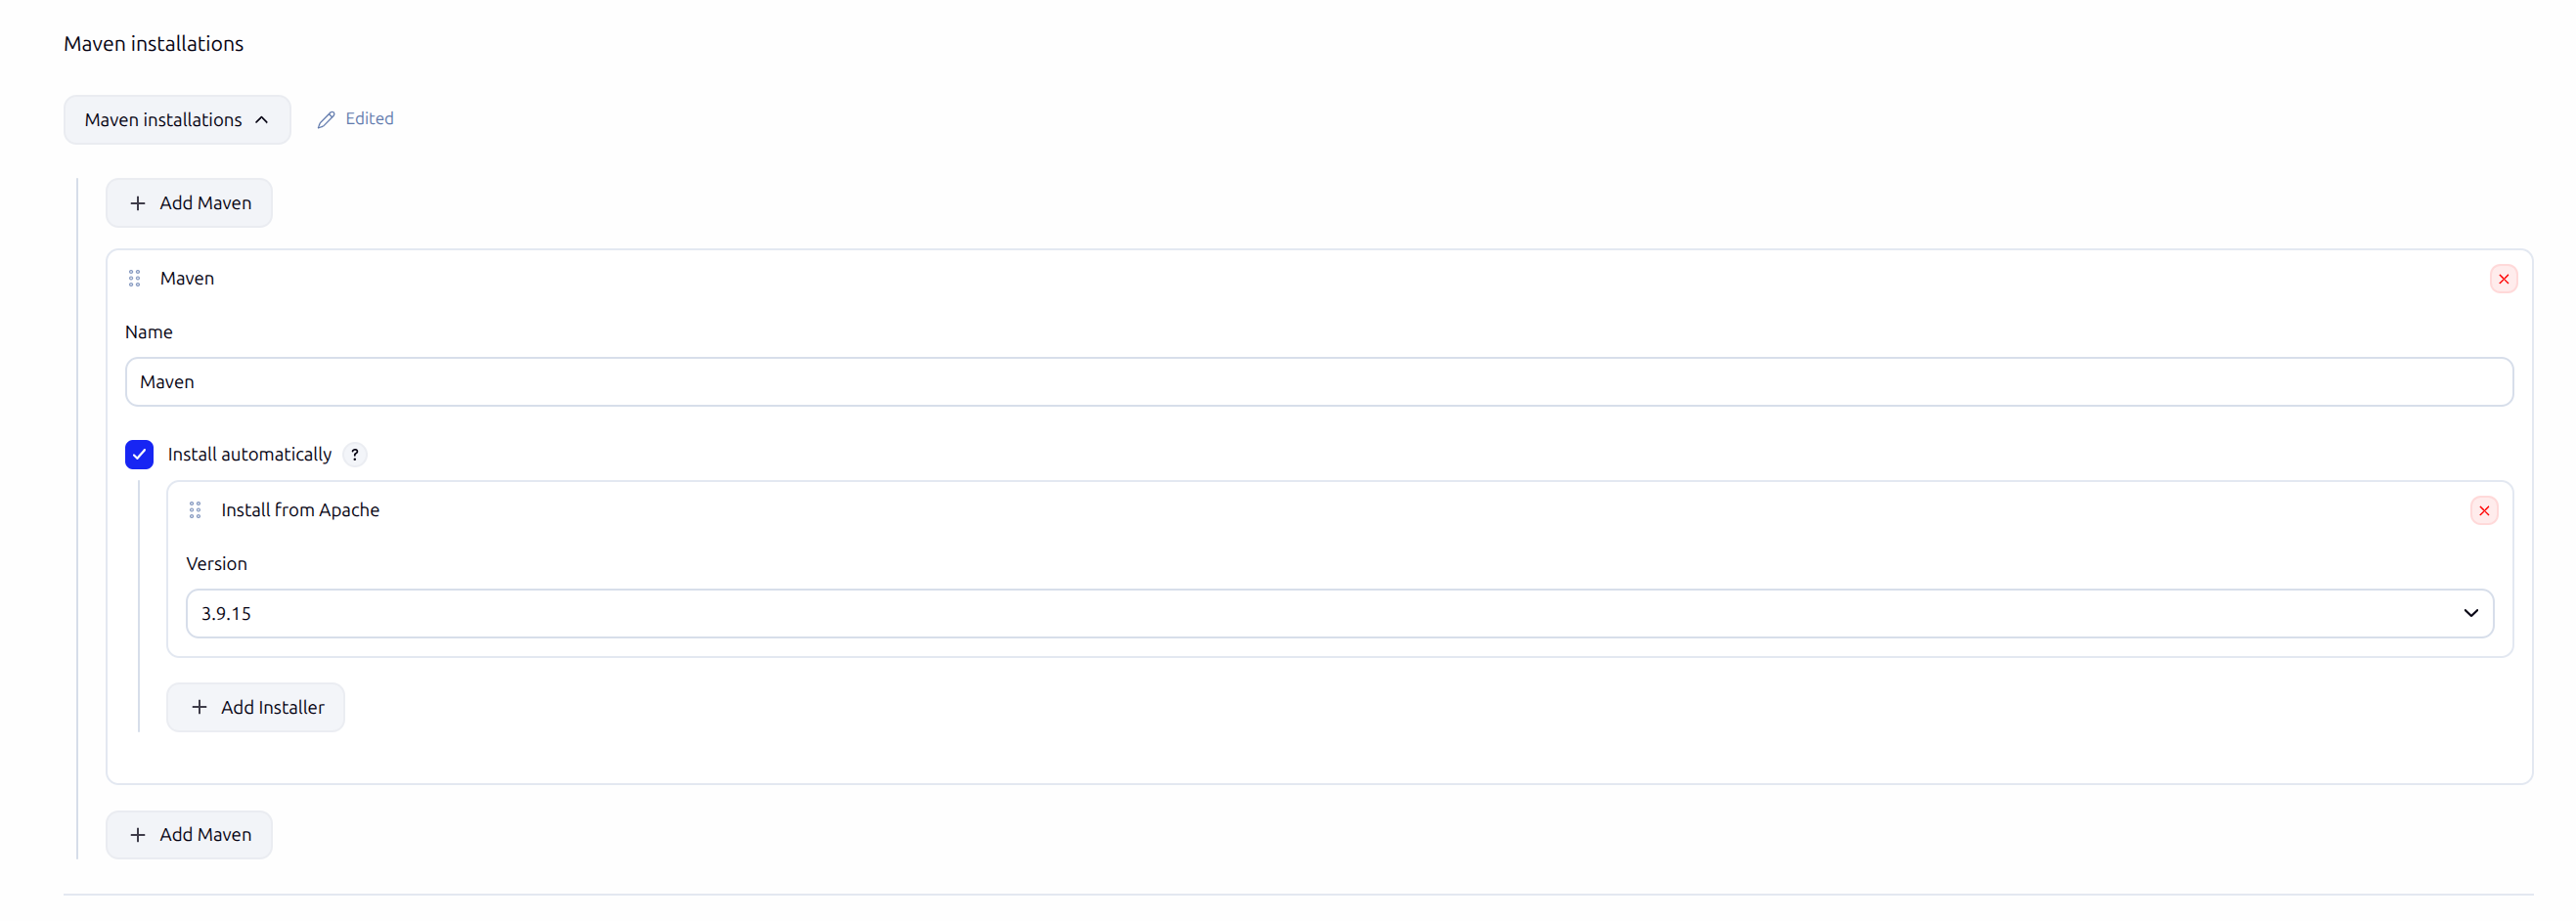
\includegraphics[width=0.9\textwidth]{img/07-jenkins-tools-maven.png}
    \caption{Cấu hình Maven trong Jenkins Global Tool Configuration}
\end{figure}

\subsection{Cấu hình Credentials}
Các credentials được lưu trong Jenkins Credentials Store:
\begin{table}[H]
\centering
\caption{Jenkins Credentials}
\begin{tabular}{|l|l|l|}
\hline
\textbf{ID} & \textbf{Loại} & \textbf{Mục đích} \\
\hline
\texttt{sonarqube-token} & Secret text & Xác thực SonarQube API \\
\hline
\texttt{snyk-token} & Secret text & Xác thực Snyk CLI \\
\hline
\end{tabular}
\end{table}

\begin{figure}[H]
    \centering
    % CHỈ DẪN ẢNH: Thả ảnh 08-jenkins-credentials-ids.png vào thư mục img/
    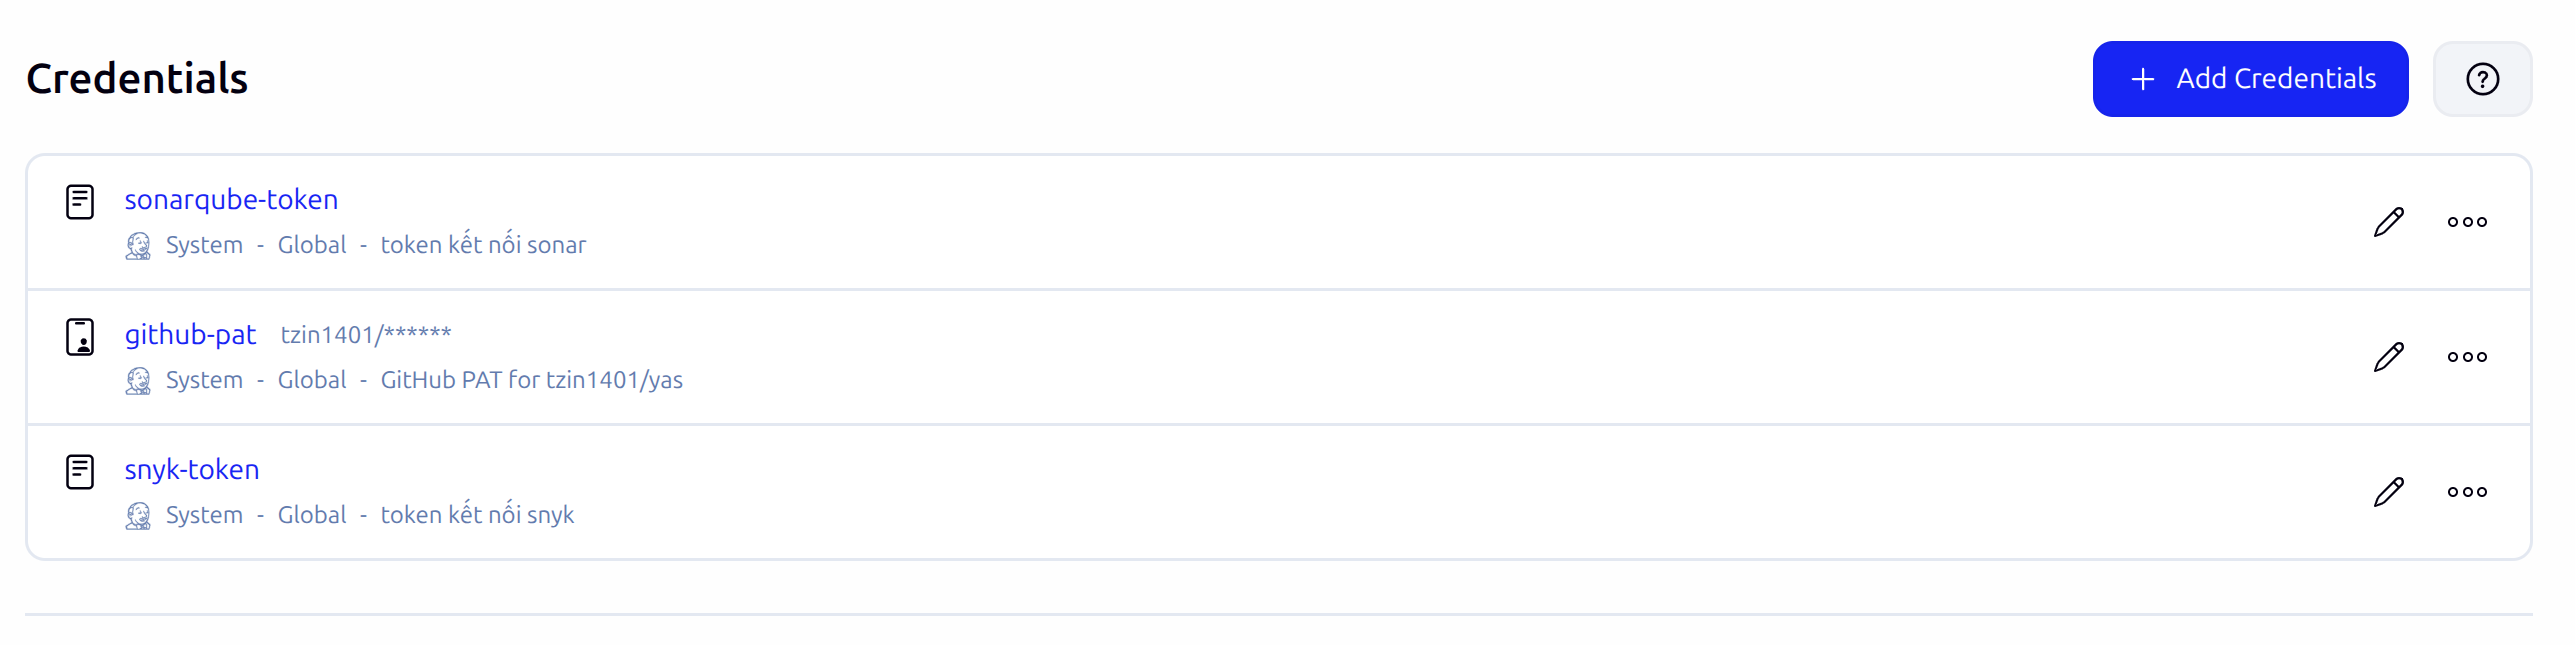
\includegraphics[width=0.9\textwidth]{img/08-jenkins-credentials-ids.png}
    \caption{Danh sách ID Credentials đã được lưu trên Jenkins}
\end{figure}

\subsection{Cấu hình Distributed Build Nodes (Agents)}
Để thực thi các tác vụ build và test một cách phân tán, nhóm đã đăng ký 3 Agent vào hệ thống Jenkins Master:
\begin{itemize}[noitemsep]
    \item \textbf{Agent-Tri}: Agent phụ trách xử lý và thực thi các build job.
    \item \textbf{Agent-QVinh}: Agent phụ trách xử lý và thực thi các build job.
    \item \textbf{Agent-TVinh}: Agent phụ trách xử lý và thực thi các build job.
\end{itemize}

\begin{figure}[H]
    \centering
    % CHỈ DẪN ẢNH: Thả ảnh 08c-jenkins-agent-nodes.png vào thư mục img/
    % Nội dung: Màn hình Manage Jenkins -> Nodes hiển thị cả 3 agent online
    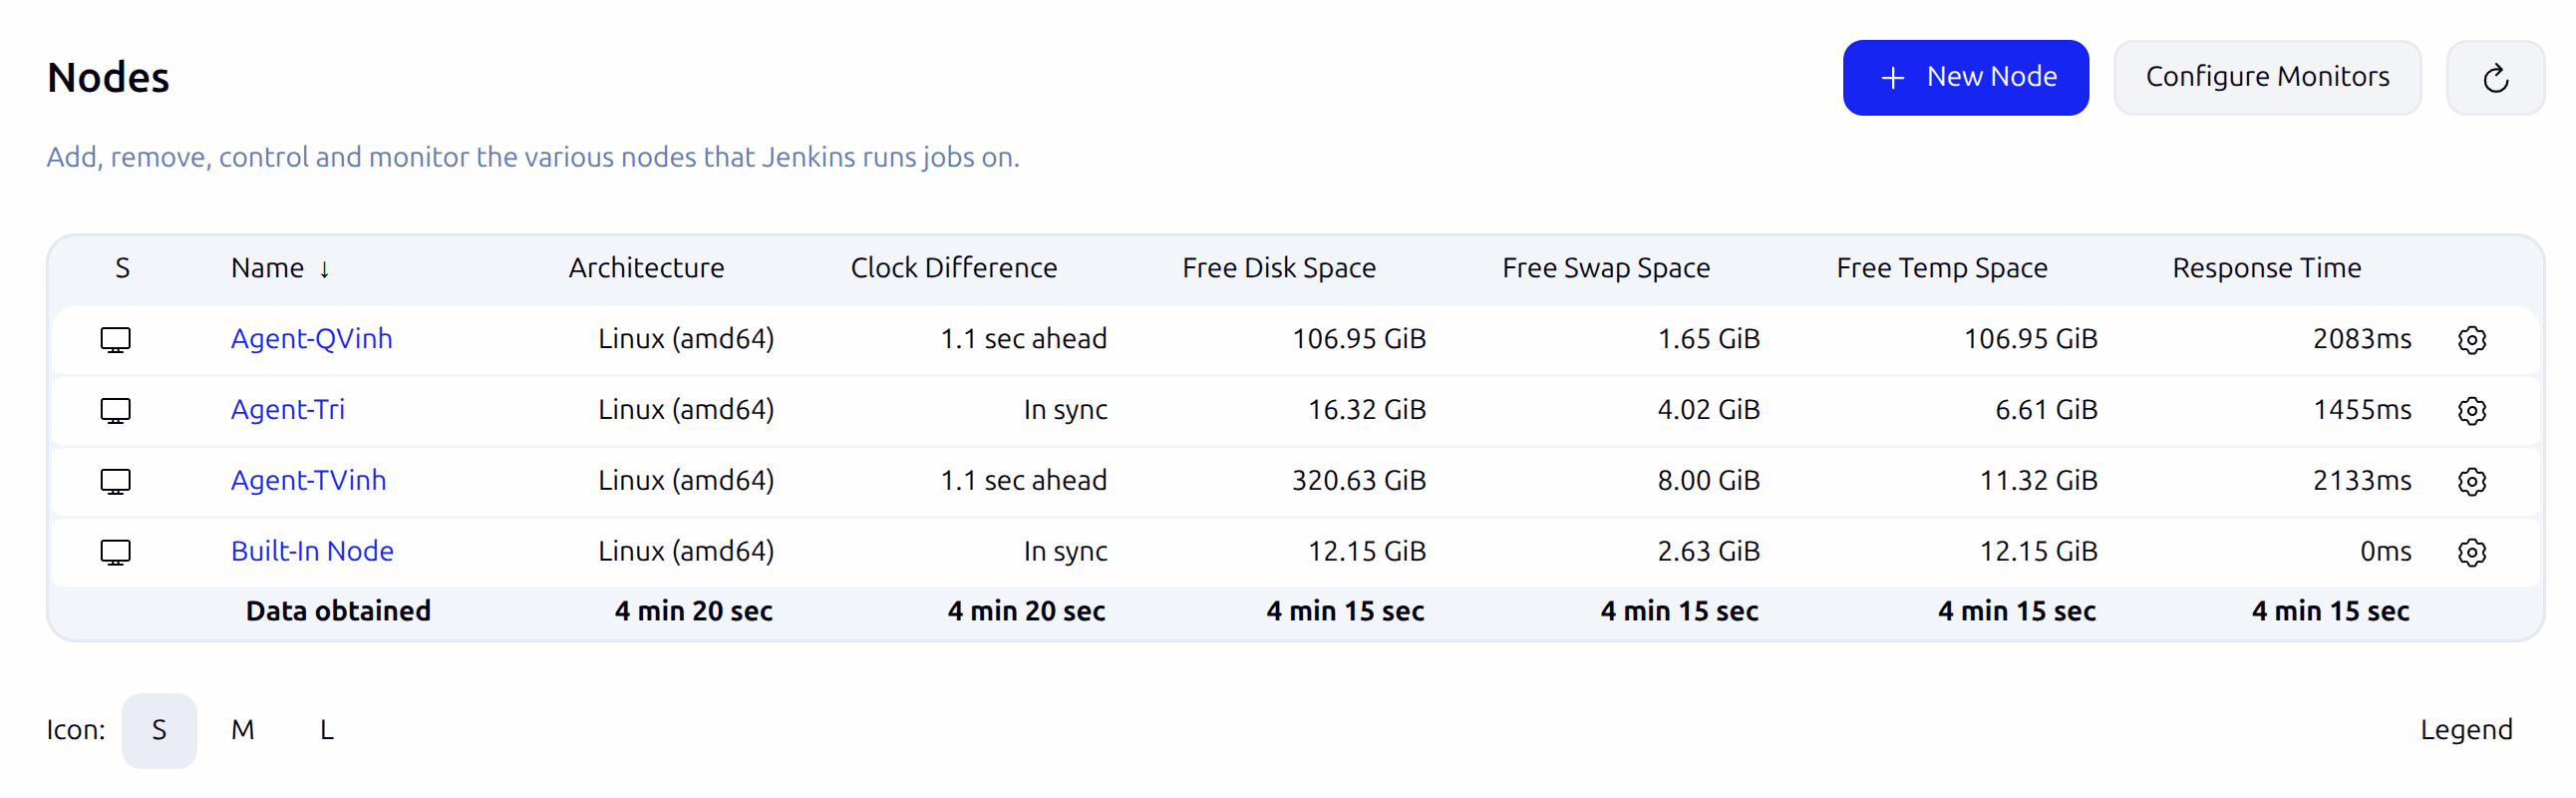
\includegraphics[width=0.9\textwidth]{img/08c-jenkins-agent-nodes.png}
    \caption{Danh sách các Nodes/Agents đã kết nối thành công với Jenkins Master}
\end{figure}

\subsubsection{Thiết lập Jenkins Agent (Node) và Cách kết nối}
Trong mô hình Distributed Build, Jenkins Master chỉ điều khiển, còn Agent (Node) là nơi thực sự chạy code.

\textbf{1.1 Các bước tạo Node trên giao diện Jenkins}:
\begin{enumerate}[noitemsep]
    \item Truy cập \textbf{Manage Jenkins} $\rightarrow$ \textbf{Nodes} $\rightarrow$ \textbf{New Node}.
    \item Đặt tên (vd: \texttt{Agent-QVinh}), chọn \textbf{Permanent Agent}.
    \item \textbf{Remote root directory}: Thư mục làm việc trên máy Agent (vd: \texttt{/home/ubuntu/jenkins-agent}).
    \item \textbf{Launch method}: Chọn \textbf{Launch agent by connecting it to the controller} (kết nối từ máy Agent đến Master qua JNLP).
\end{enumerate}

\textbf{1.2 Cách kết nối từ máy Agent đến Node (Master)}:
Sau khi nhấn Save, Jenkins sẽ cung cấp một đoạn mã lệnh. Nhóm tiến hành SSH vào máy Agent và thực hiện:
\begin{enumerate}[noitemsep]
    \item Tải file \texttt{agent.jar}:
\begin{lstlisting}[language=bash]
curl -sO http://<IP-Jenkins-Master>:8080/jnlpJars/agent.jar
\end{lstlisting}
    \item Chạy lệnh kết nối:
\begin{lstlisting}[language=bash]
java -jar agent.jar -url http://<IP-Jenkins-Master>:8080/ -secret <SECRET_KEY> -name "Agent-QVinh" -workDir "/home/ubuntu/jenkins-agent"
\end{lstlisting}
    \item \textit{Lưu ý}: Để Agent tự khởi chạy lại khi khởi động máy, nhóm cấu hình lệnh này thành một Systemd Service trên Linux.
\end{enumerate}

\subsubsection{Cài đặt môi trường thực thi (Tooling) trên Agent}
Để chạy được toàn bộ Pipeline ``yas'', các máy Agent (Node) được cài đặt các công cụ sau:
\begin{itemize}[noitemsep]
    \item \textbf{Docker Engine \& Docker Compose}: Cài đặt để thực hiện Stage Build Image và quét Snyk Container. Đồng thời, chạy lệnh \texttt{sudo usermod -aG docker jenkins} và khởi động lại Agent để user Jenkins có quyền thực thi lệnh Docker.
    \item \textbf{Java Development Kit (JDK)}: Cài đặt phiên bản khớp với dự án (ví dụ JDK 25) để thực thi file \texttt{agent.jar} và chạy Maven.
    \item \textbf{Apache Maven}: Cài đặt để chạy lệnh \texttt{mvn test}, \texttt{mvn dependency:tree} và các lệnh kiểm tra coverage.
    \item \textbf{Git}: Cài đặt để Agent có thể thực hiện Stage Checkout code từ GitHub.
\end{itemize}

\subsubsection{Cấu hình Snyk Auth trên Terminal của Agent}
Trong môi trường CI/CD, việc xác thực Agent bằng Token là tối ưu nhất.

\begin{enumerate}[noitemsep]
    \item \textbf{Cài đặt Snyk CLI}: Agent cài đặt Snyk thông qua lệnh \texttt{npm install -g snyk}.
    \item \textbf{Xác thực bằng Token}: Trên Terminal của Agent, chạy lệnh: \texttt{snyk auth <YOUR\_SNYK\_API\_TOKEN>} hoặc gán biến môi trường \texttt{SNYK\_TOKEN} để Snyk tự động nhận diện.
\end{enumerate}

\begin{figure}[H]
    \centering
    % CHỈ DẪN ẢNH: Thả ảnh 09b-snyk-auth-agent.png vào thư mục img/
    % Nội dung: Chụp màn hình terminal gõ lệnh auth và hiển thị thành công "Your account has been successfully authenticated"
    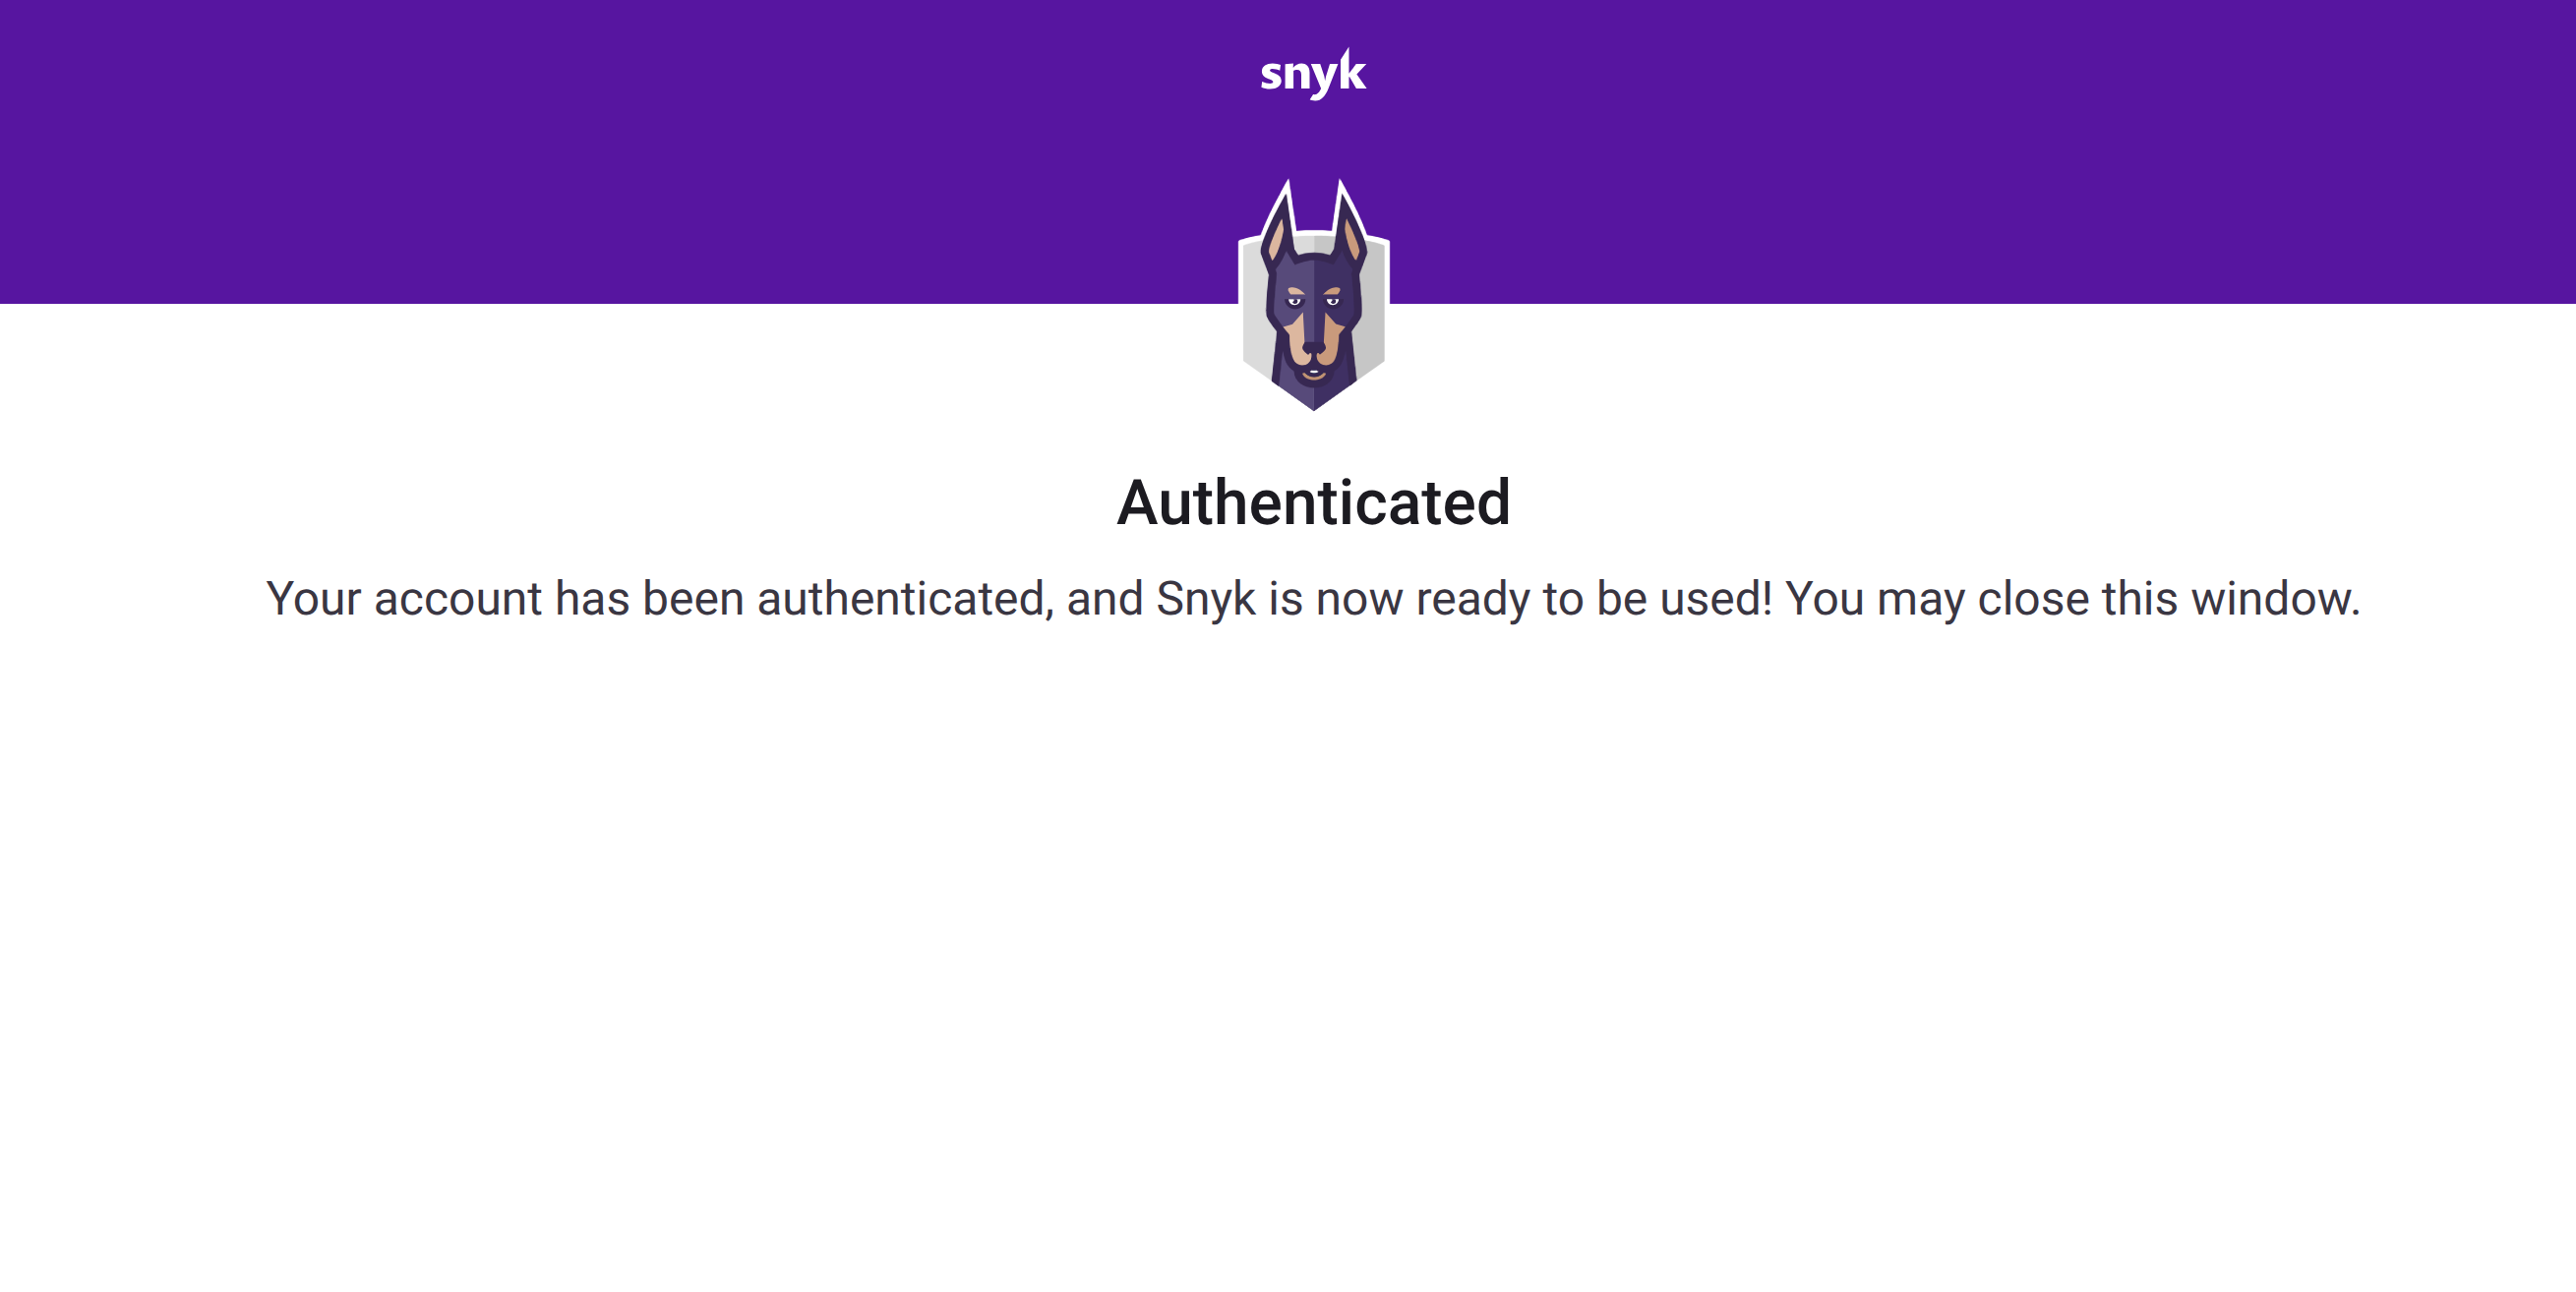
\includegraphics[width=0.9\textwidth]{img/09b-snyk-auth-agent.png}
    \caption{Xác thực tài khoản Snyk thành công trên Agent}
\end{figure}

\subsection{Cấu hình hiển thị Biểu đồ và Thống kê (Plugins)}
Để Jenkins hiển thị được các tab báo cáo và biểu đồ từ kết quả quét, nhóm đã cấu hình các Plugin sau trên Master:

\begin{itemize}
    \item \textbf{JaCoCo Plugin}: Sau khi chạy \texttt{mvn jacoco:report}, plugin này đọc file \texttt{.exec} trong thư mục target để hiển thị biểu đồ Coverage Trend ngay tại trang chủ của Job.
\end{itemize}

\begin{figure}[H]
    \centering
    % CHỈ DẪN ẢNH: Thả ảnh 10b-jenkins-jacoco-coverage-trend.png vào thư mục img/
    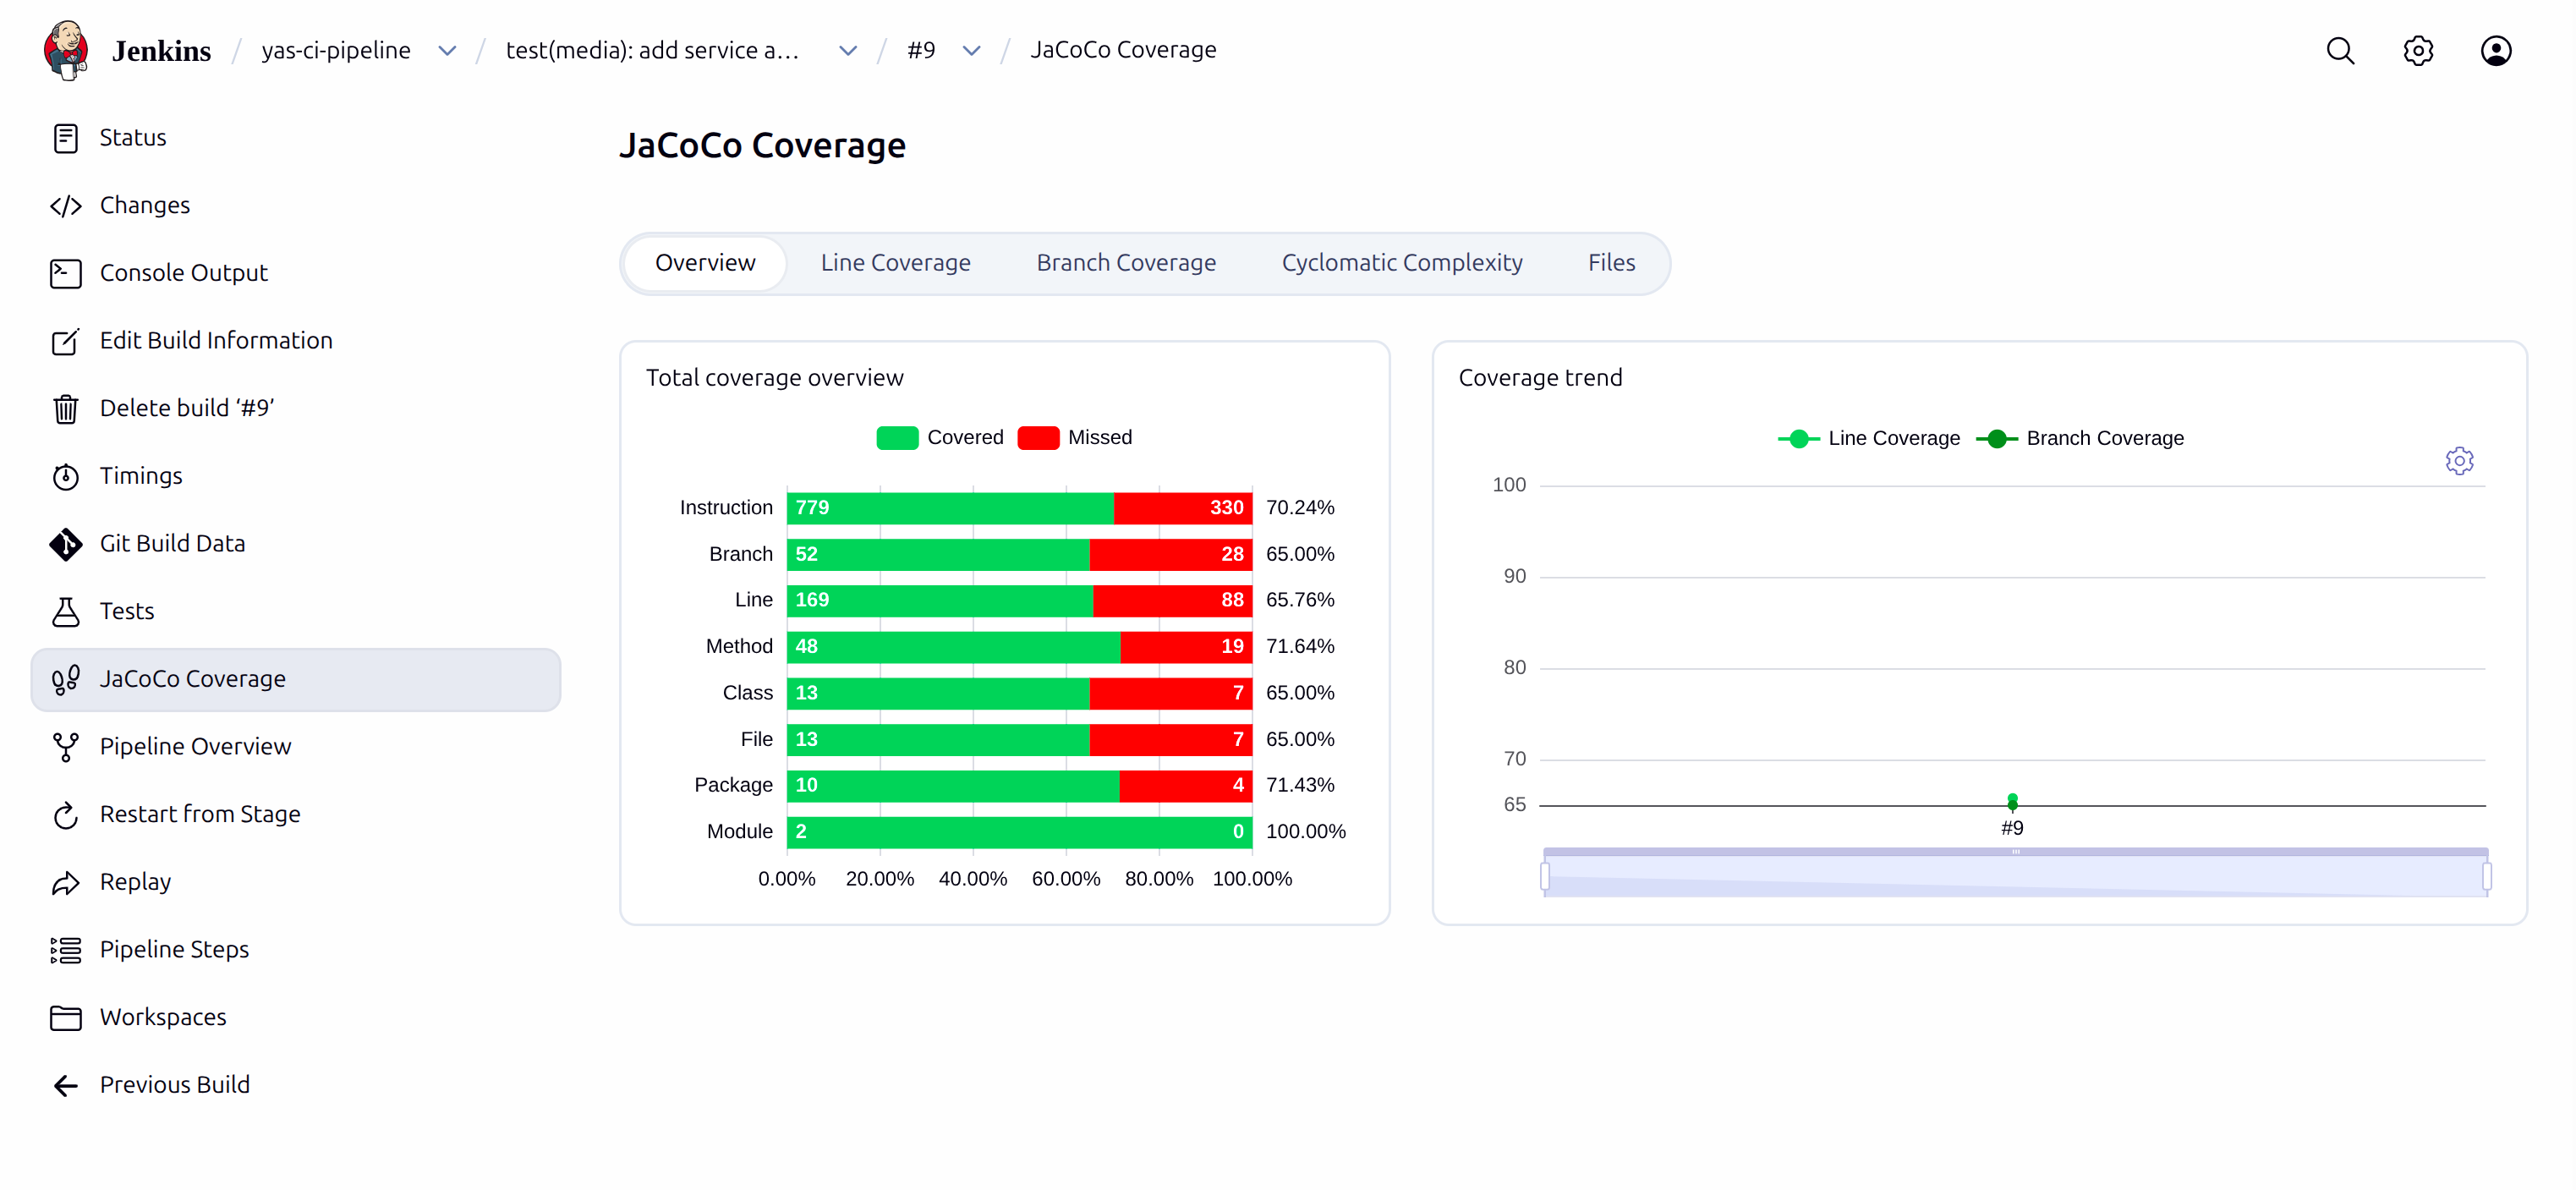
\includegraphics[width=0.9\textwidth]{img/10b-jenkins-jacoco-coverage-trend.png}
    \caption{Biểu đồ Coverage Trend hiển thị thông qua JaCoCo Plugin}
\end{figure}

\begin{itemize}
    \item \textbf{SonarQube Scanner Plugin}: Cấu hình Webhook trỏ về \texttt{/sonarqube-webhook/} để hiển thị trạng thái Quality Gate (Passed/Failed) trực tiếp trên Pipeline.
\end{itemize}

\begin{figure}[H]
    \centering
    % CHỈ DẪN ẢNH: Thả ảnh 08b-jenkins-system-sonarqube-server.png vào thư mục img/
    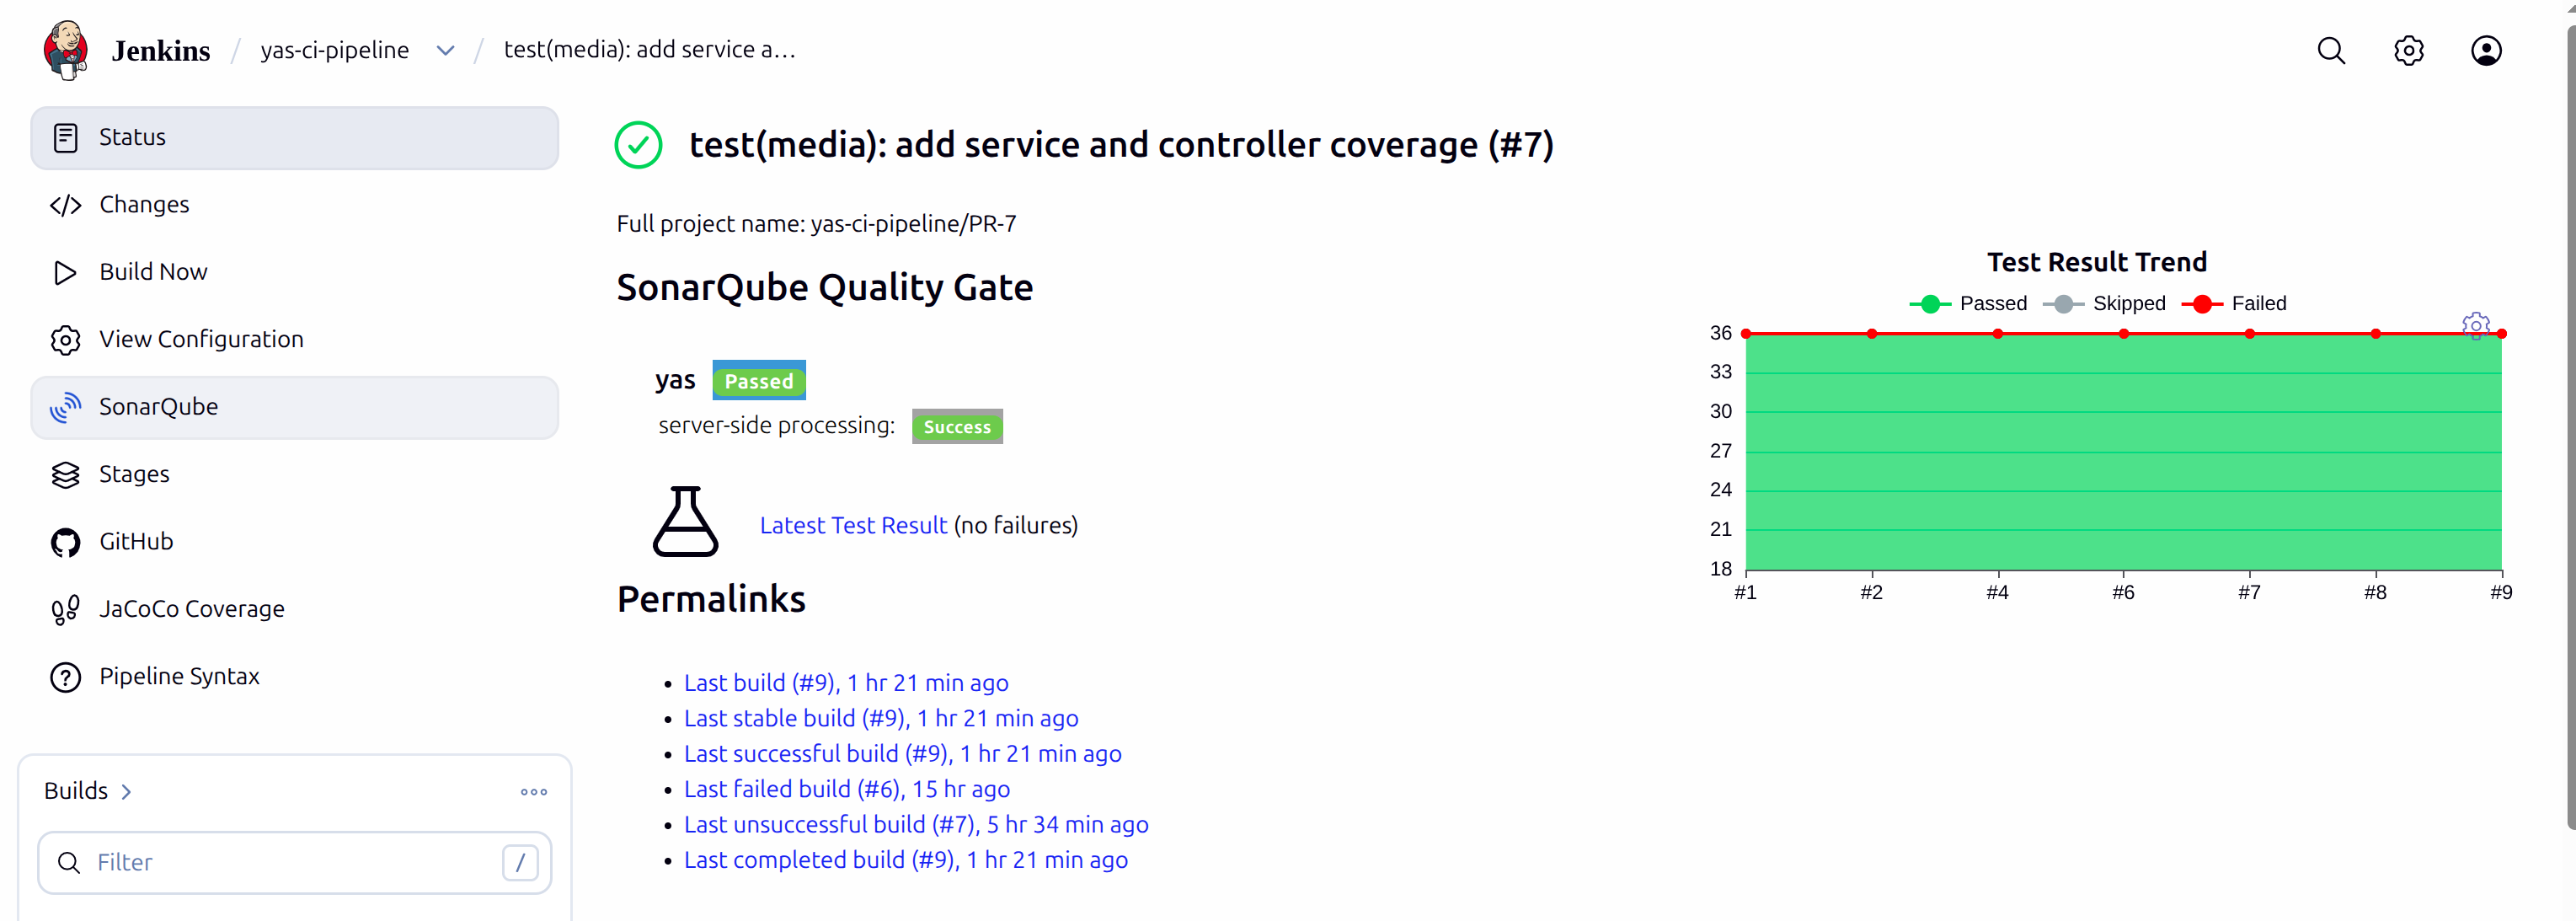
\includegraphics[width=0.9\textwidth]{img/08b-jenkins-system-sonarqube-server.png}
    \caption{Thống kê của SonarQube}
\end{figure}

\begin{itemize}
    \item \textbf{Snyk Security Plugin}: Cho phép xem chi tiết các lỗ hổng (Vulnerabilities) theo mức độ nghiêm trọng (High, Medium, Low) ngay trong giao diện Jenkins.
\end{itemize}

\subsection{Tạo Multibranch Pipeline Job}
Nhóm tạo job \texttt{yas-ci-pipeline} với loại \textbf{Multibranch Pipeline}:

\begin{enumerate}[noitemsep]
    \item \textbf{Branch Sources}: GitHub repository \texttt{tzin1401/yas}
    \item \textbf{Discover branches}: Strategy ``Exclude branches that are also filed as PRs'' --- tránh build trùng lặp khi branch đã có PR
    \item \textbf{Discover pull requests from origin}: Merging the pull request with the current target branch revision
    \item \textbf{Build Configuration}: Jenkinsfile tại root của repository
    \item \textbf{Scan Repository Triggers}: Tự động quét mỗi khi có webhook từ GitHub
\end{enumerate}

\begin{figure}[H]
    \centering
    % CHỈ DẪN ẢNH: Thả ảnh 04-jenkins-config-branch-sources.png vào thư mục img/
    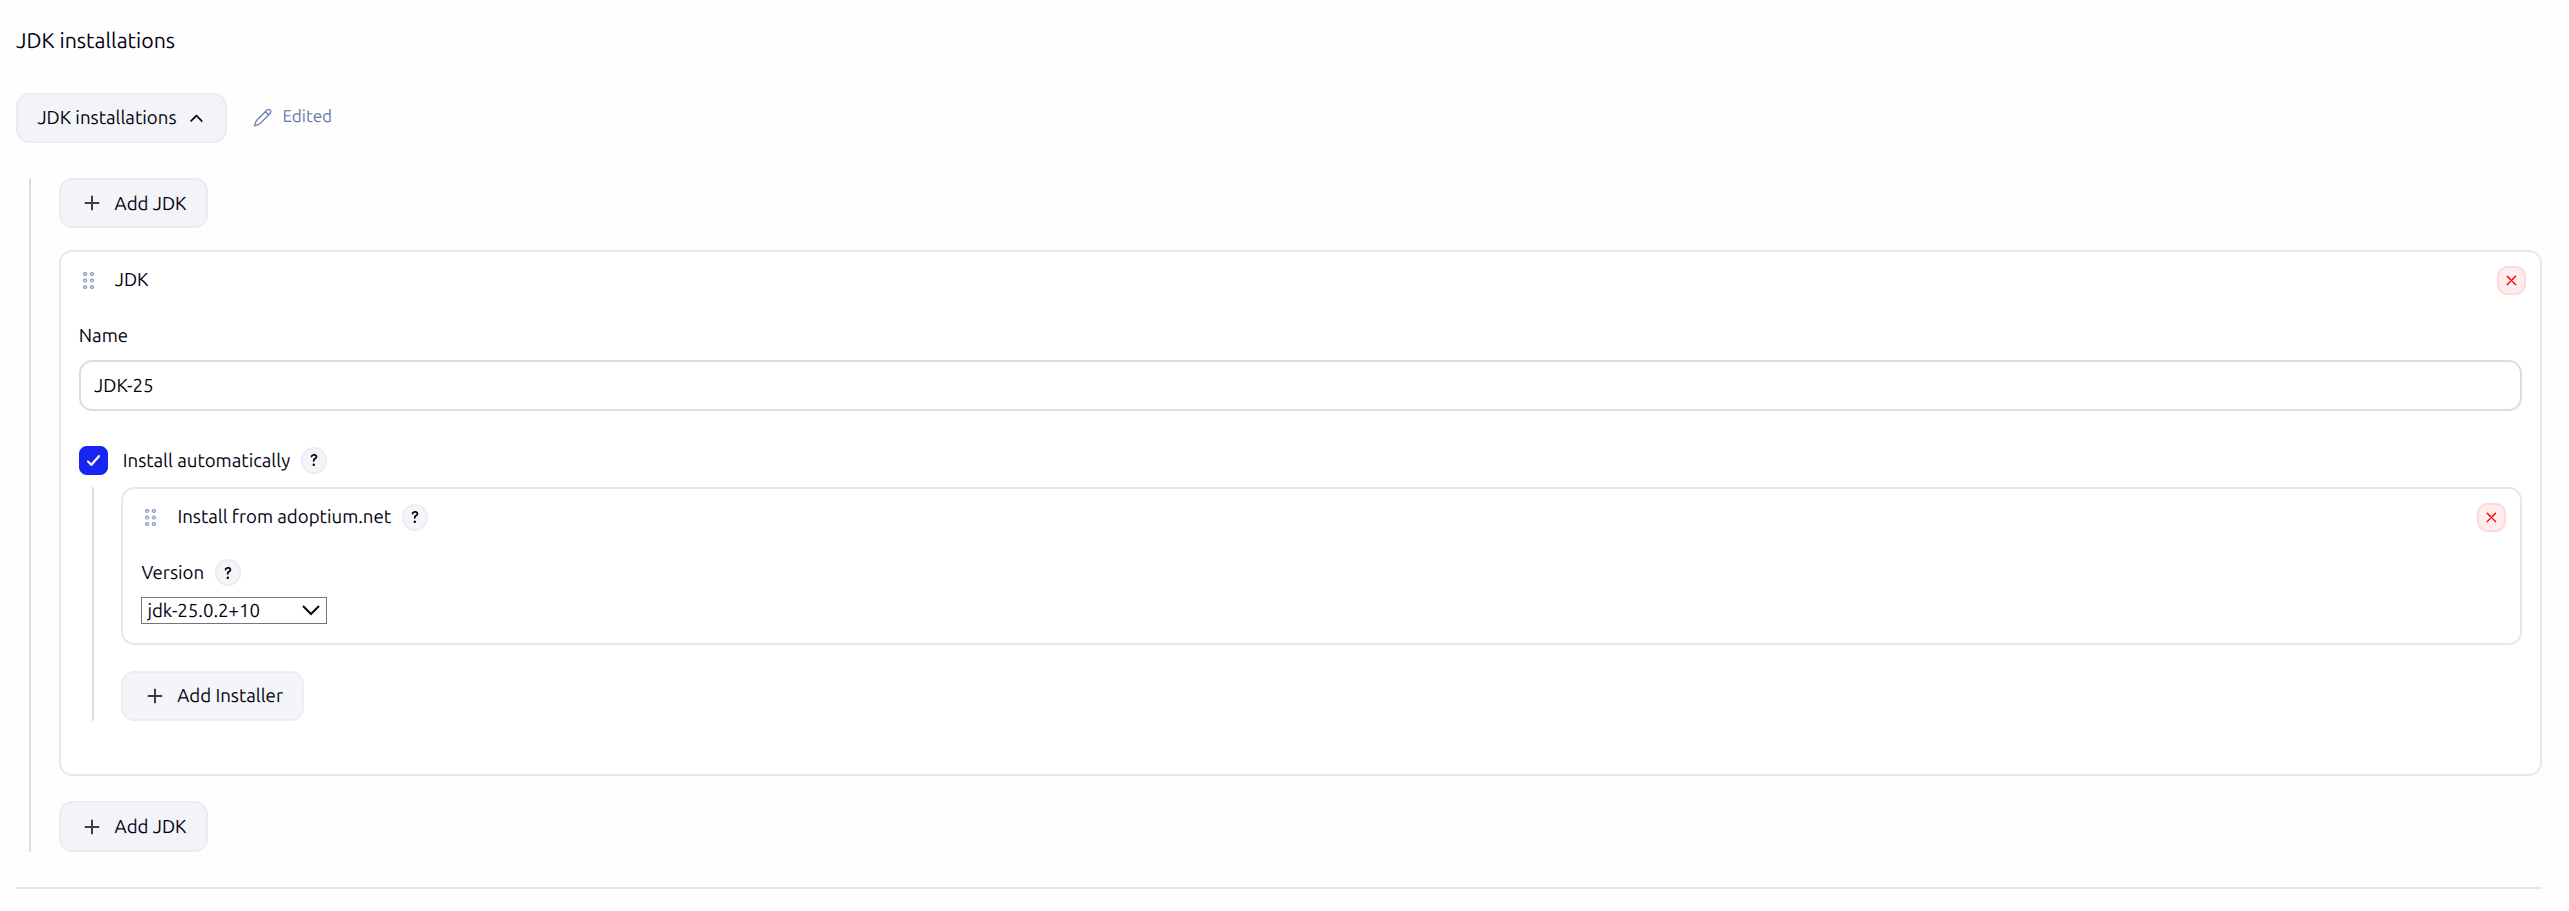
\includegraphics[width=0.9\textwidth]{img/04-jenkins-config-branch-sources.png}
    \caption{Cấu hình Branch Sources trong Multibranch Pipeline Job}
\end{figure}

\begin{figure}[H]
    \centering
    % CHỈ DẪN ẢNH: Thả ảnh 05-jenkins-config-jenkinsfile-path.png vào thư mục img/
    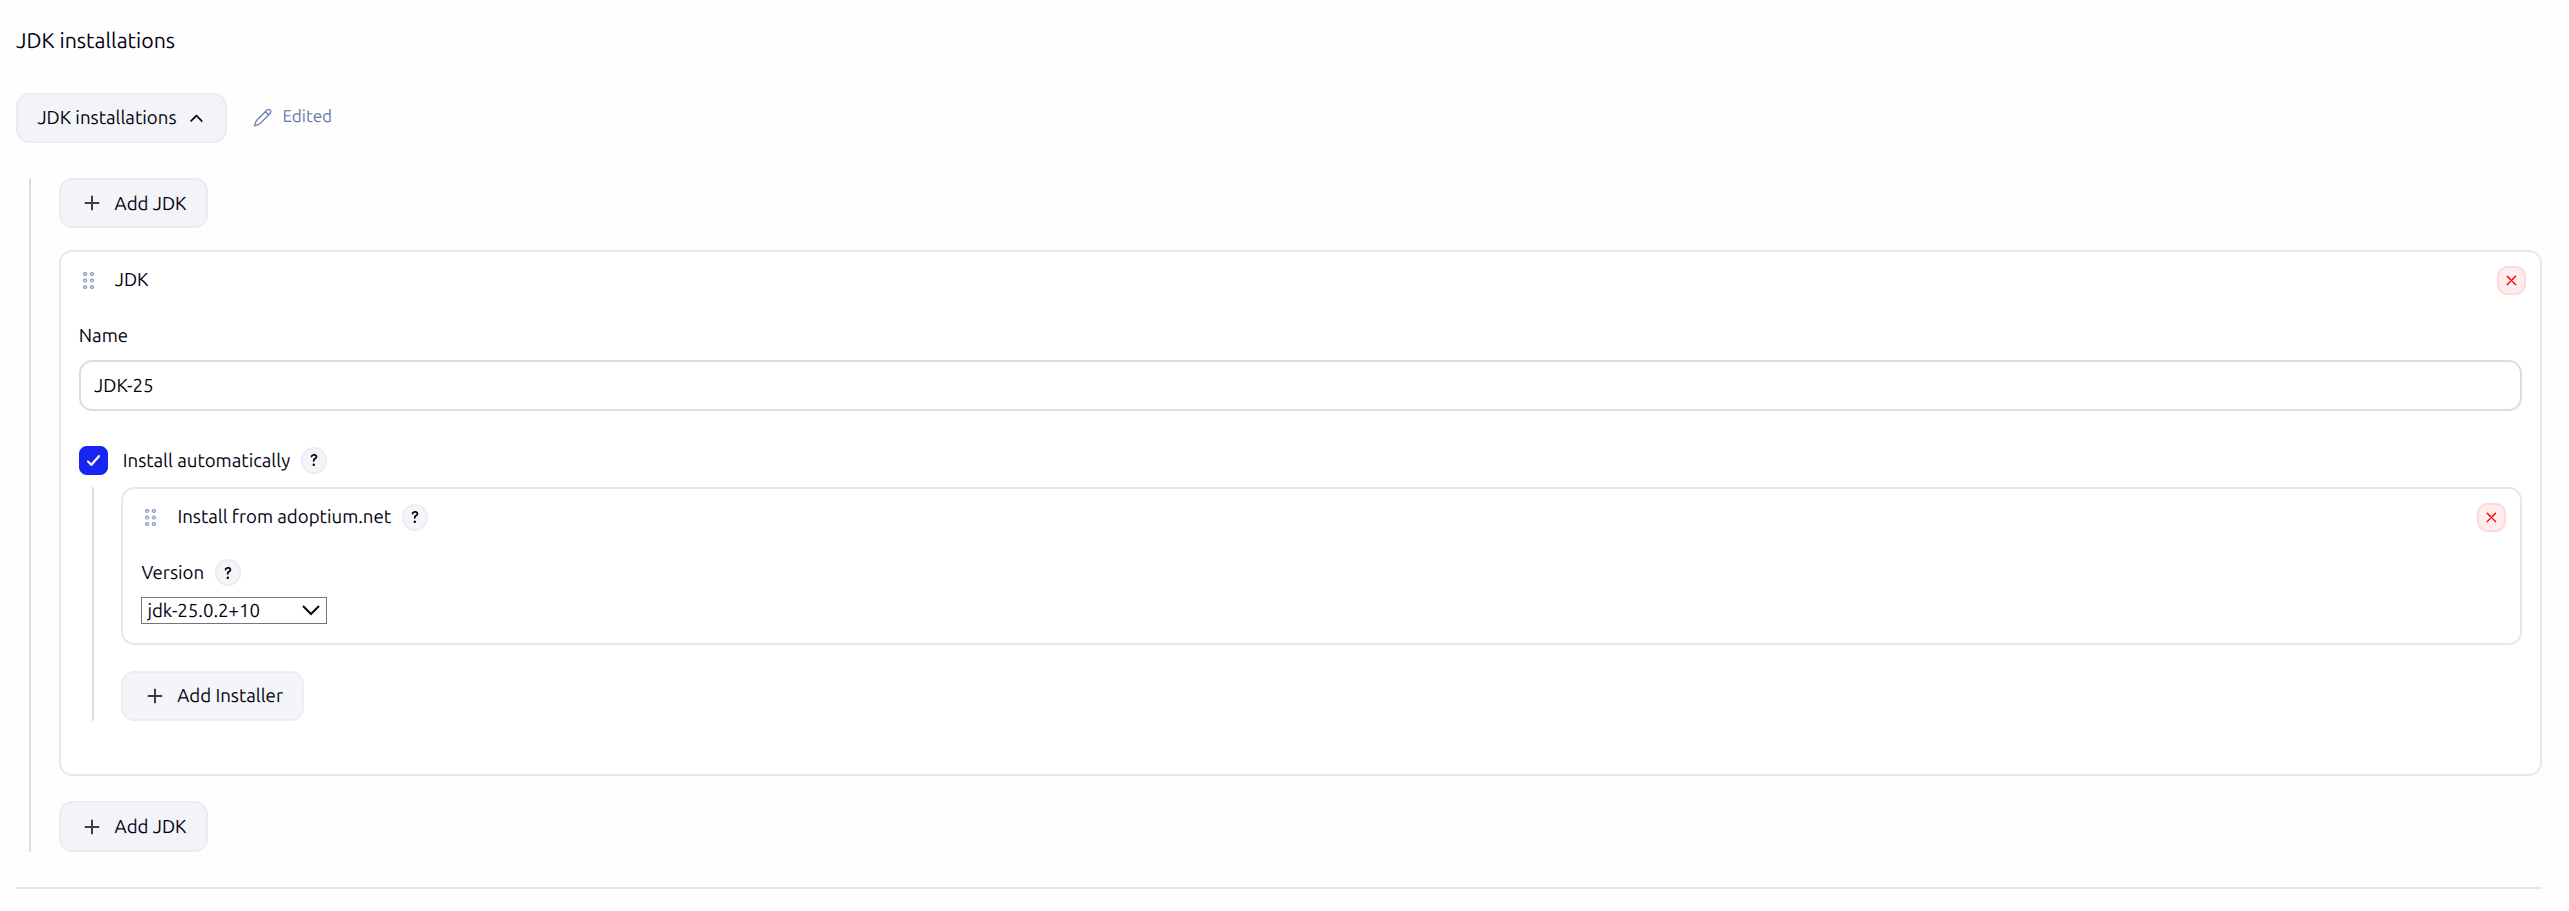
\includegraphics[width=0.9\textwidth]{img/05-jenkins-config-jenkinsfile-path.png}
    \caption{Cấu hình đường dẫn Jenkinsfile trong Multibranch Pipeline Job}
\end{figure}

\subsection{Kết quả: Jenkins tracking branches và PRs}
Sau khi cấu hình, Jenkins tự động phát hiện và tracking:
\begin{itemize}[noitemsep]
    \item \textbf{5 branches}: main, ci/setup-jenkins-pipeline, feature/media-tests, tri/tax-tests, test/ci-path-filter
    \item \textbf{5 pull requests}: PR \#3, \#4, \#5, \#6, \#7
\end{itemize}

\begin{figure}[H]
    \centering
    % CHỈ DẪN ẢNH: Thả ảnh 02-jenkins-multibranch-branches.png vào thư mục img/
    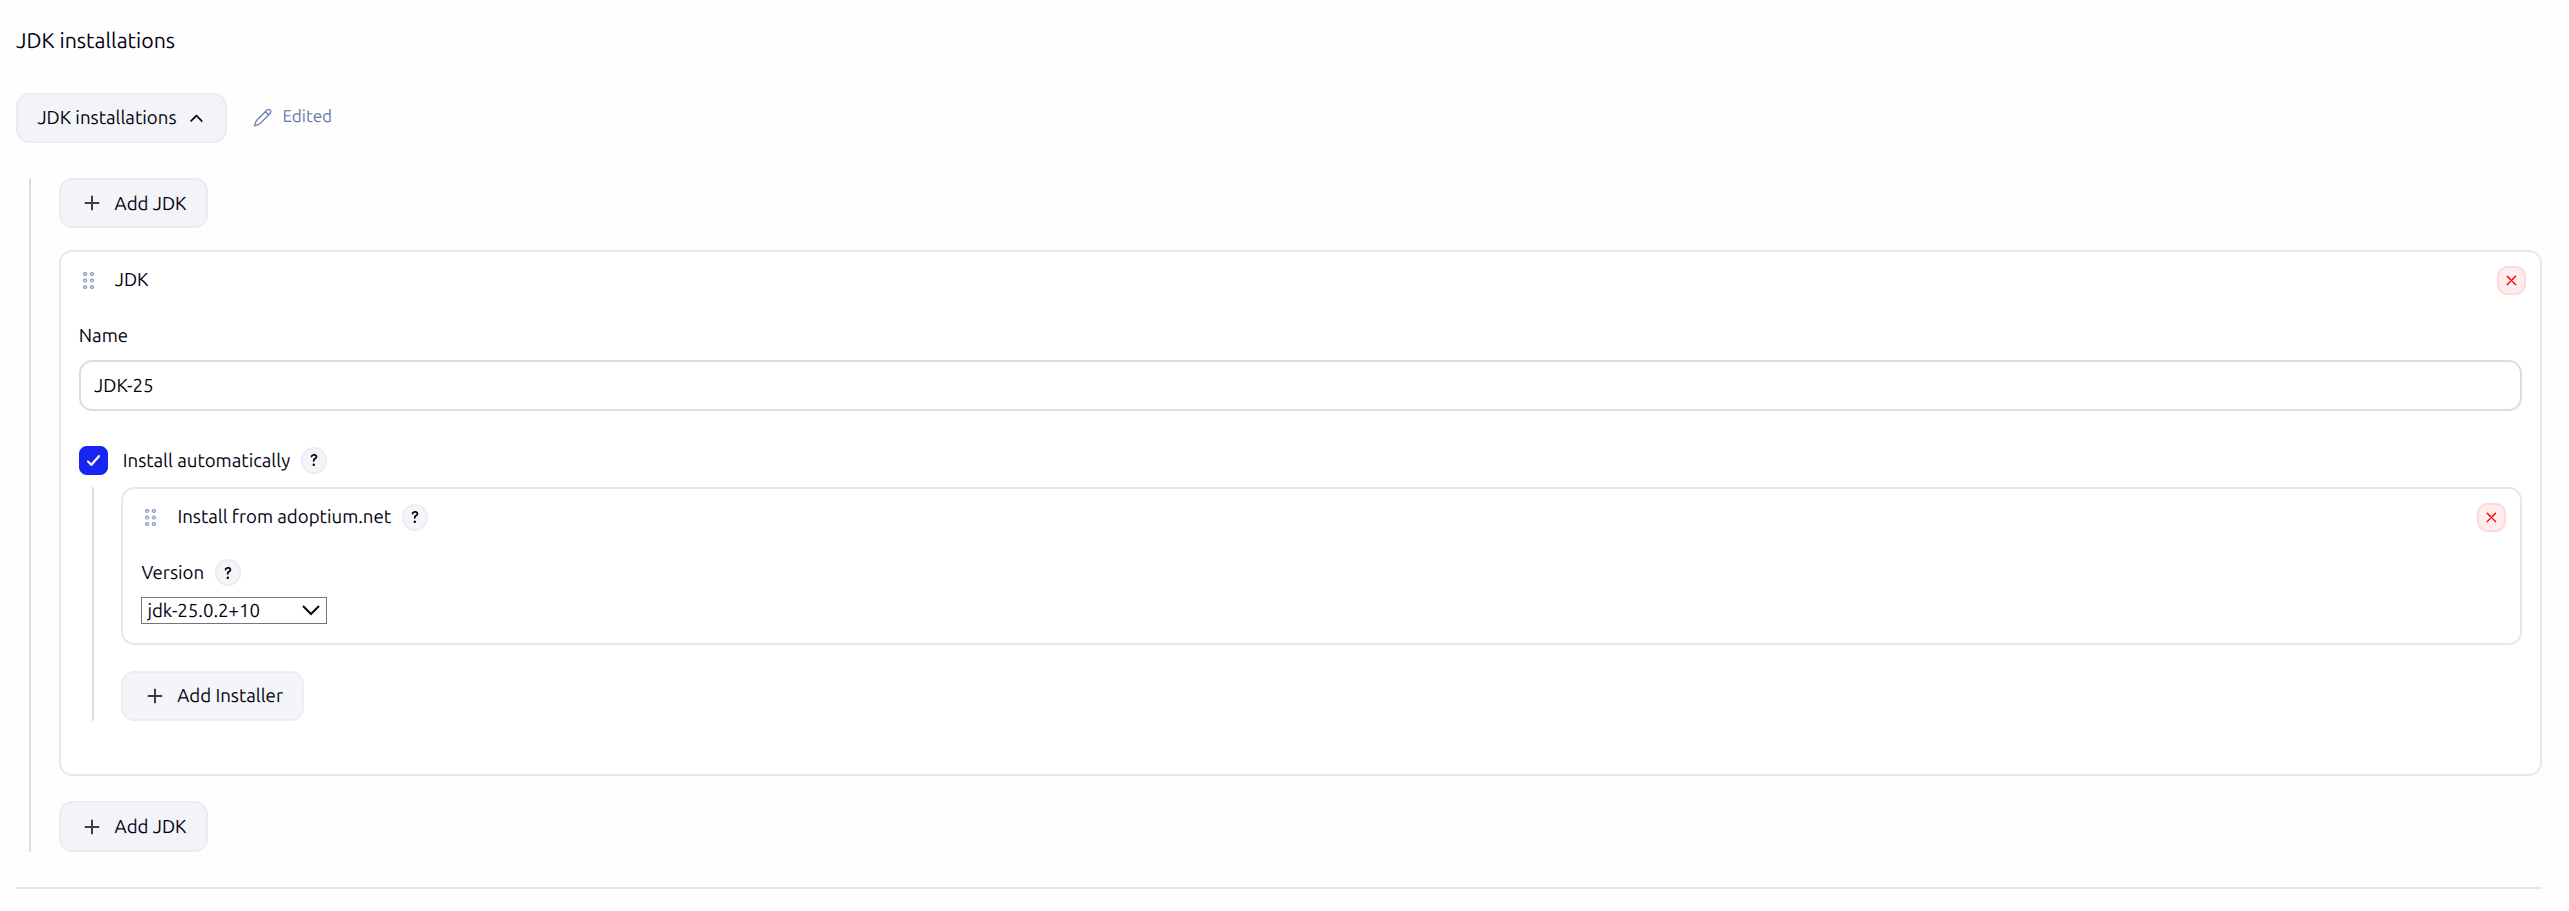
\includegraphics[width=0.9\textwidth]{img/02-jenkins-multibranch-branches.png}
    \caption{Danh sách các nhánh được tự động phát hiện và build}
\end{figure}

\begin{figure}[H]
    \centering
    % CHỈ DẪN ẢNH: Thả ảnh 03-jenkins-multibranch-prs.png vào thư mục img/
    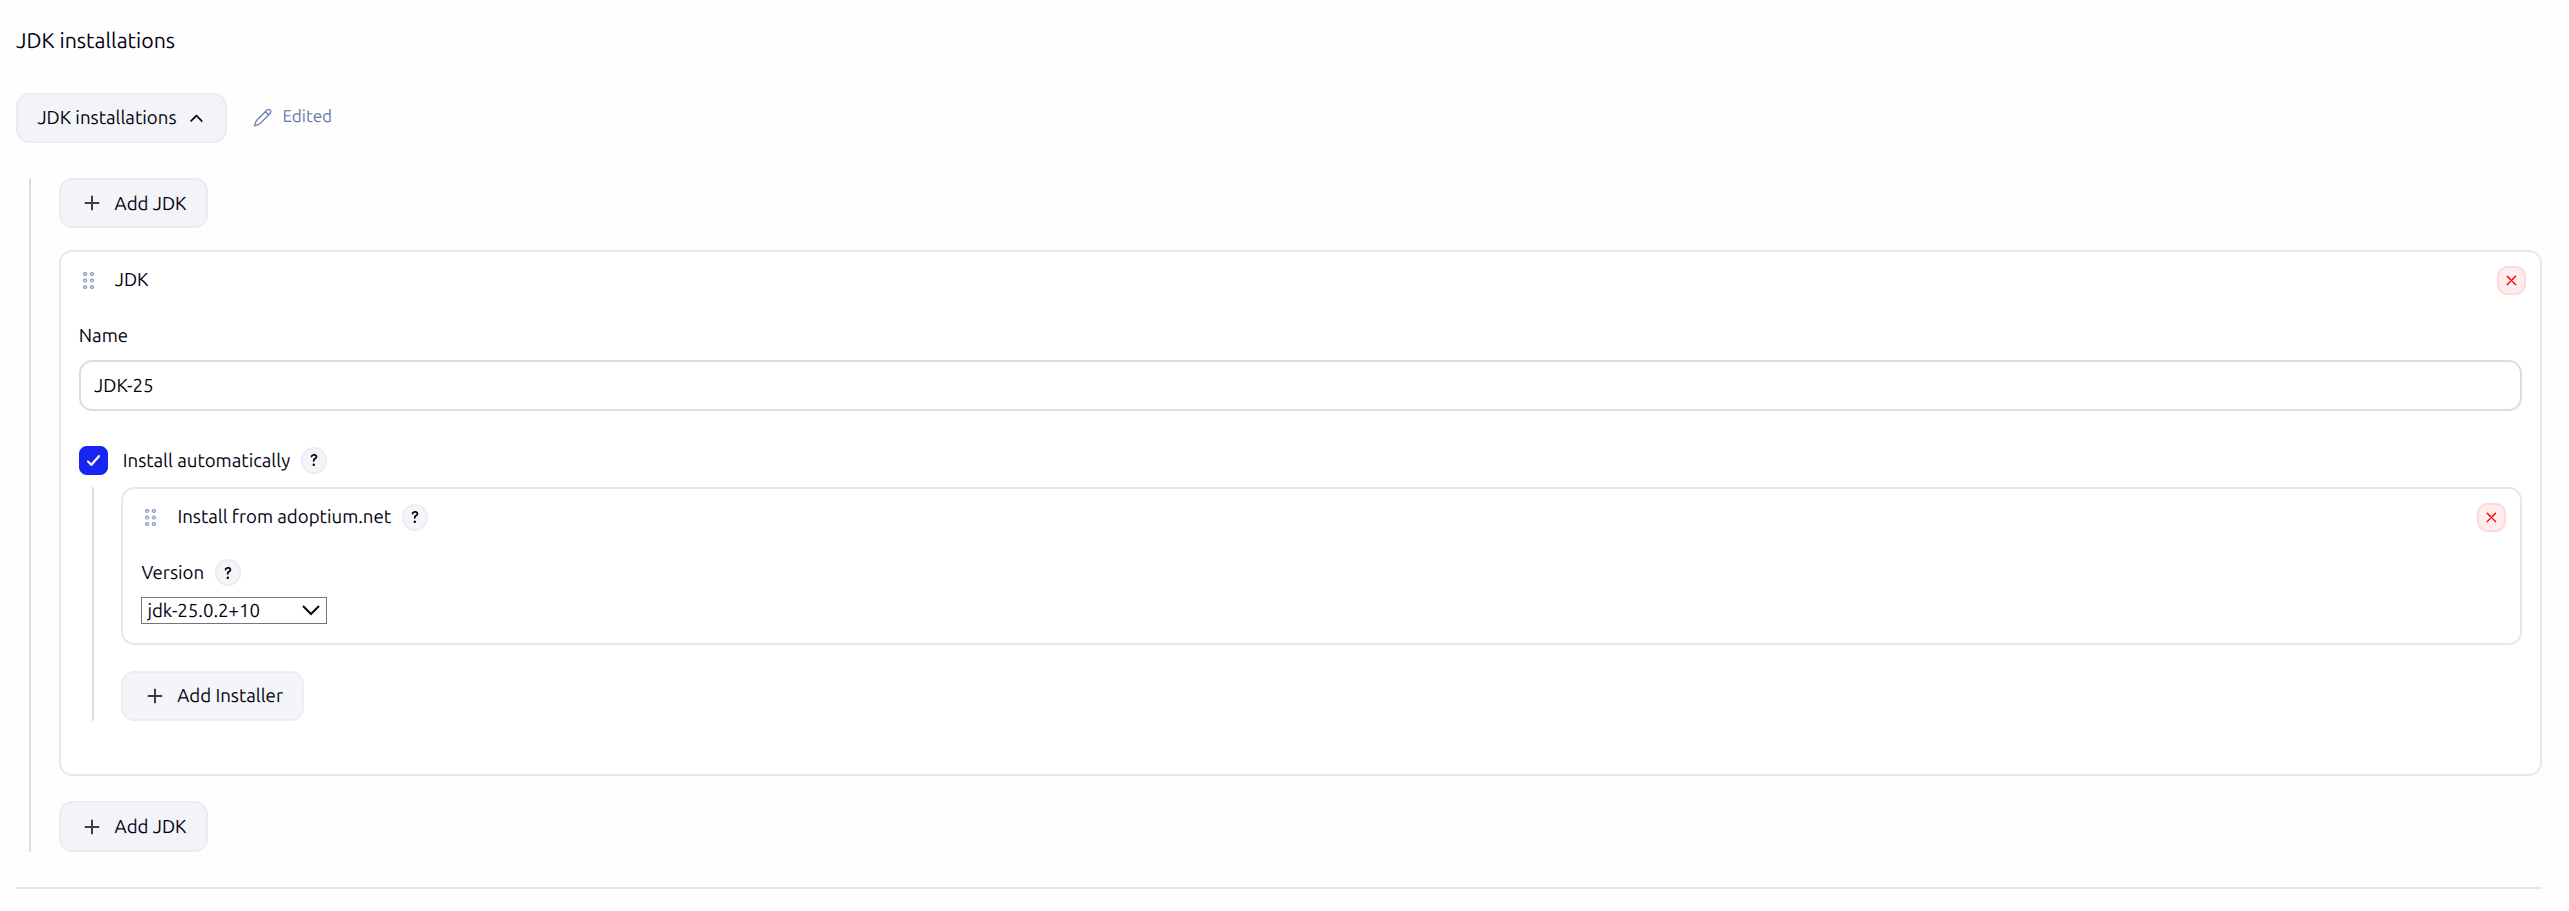
\includegraphics[width=0.9\textwidth]{img/03-jenkins-multibranch-prs.png}
    \caption{Danh sách các Pull Request được tự động phát hiện và build}
\end{figure}
